\section{Imagen}
\label{sec:imagen}

Imagen \cite{imagen} is a text-to-image diffusion model that builds on the power of large transformer language models \cite{transformer} (LLMs) to generate high-fidelity images. The combination of diffusion (section \ref{subsec:diffusion_models}) and LLMs have shown remarkable outputs. One of the main observation in the paper that the researchers discovered is that a \textbf{large frozen LLM has bigger impact on the fidelity of generated images than increasing the amount of parameters in the image diffusion model}. Another contribution in the paper is the introduction of new benchmark called \textbf{DrawBench} to evaluate text-to-image models such as DALL-E \cite{dalle}, VQ-GAN+CLIP \cite{vqgan_clip}, latent diffusion models \cite{stable_diffusion}, GLIDE \cite{glide}, and DALL-E 2 \cite{dalle_2}.

The researchers achieved a new state-of-the-art COCO FID score of 7.27, and human raters prefer Imagen in terms of image-text alignment with reference images. On DrawBench the researchers found Imagen outperforms state-of-the-art DALL-E 2 model in human evaluation on text-to-image task. But most importantly, the use of large pre-trained frozen language models was found to be instrumental to both image fidelity and image-text alignment.

There are five main contributions in the paper:

\begin{enumerate}
    \item \textbf{Effectiveness of large frozen text encoders}: large frozen language models that were trained only on text data have a significant impact on the fidelity of generated images compared to increasing the parameters of the diffusion image model. Scaling the language model is easy, since unlabeled text data is abundant and available on the internet.
    \item \textbf{Dynamic thresholding}: is a new sampling technique that improves image fidelity and text-image alignment, which improves upon static thresholding. We will take a look at this in more detail in the following sections (section \ref{subsec:imagen_diffusion_guidance_weight}).
    \item \textbf{Effective U-Net}: a new U-Net architecture that is simpler and more memory efficient.
    \item \textbf{COCO FID score of 7.27}: imagen achieved a new state-of-the-art COCO FID score of 7.27, which outperforms all other previous works.
    \item \textbf{DrawBench}: a new evaluation benchmark for text-to-image task. Imagen outperforms all other works, including DALL-E 2 \cite{dalle_2} on this benchmark.
\end{enumerate}



















\subsection{Text-to-Text Transfer Transformer (T5)}

\textbf{T}ext-\textbf{t}o-\textbf{T}ext \textbf{T}ransfer \textbf{T}ransformer (T5) \cite{t5_model} is a model that was introduced by Google Research that treats tasks as a text-to-text problems. For example, for summarization tasks we could prompt the LLM: "Please summarize the following: ...", for translation tasks we could prompt the LLM: "Translate from English to French the word 'You'", as well as for text classification, question answering, conversations, and other tasks. In short, this knowledge can be viewed as developing a 'general-purpose' model that can understand text.  Instead of explicitly training the model to learn words or text, such as in the case of \textbf{word vectors} \cite{cbow_word2vec}, a more common practice is to \textbf{pre-train} \cite{bert} the model on data-rich task in an unsupervised manner. The model T5 is open-source and was trained on large corpora of textual data. The base version of the model (T5-base) consists of 220 million parameters, while the largest version of the model (T5-XXL) consists of \textbf{11 billion parameters}. In the context of Imagen, the Imagen model uses a frozen version of T5-XXL model to encode conditional text prompts.

This pre-training approach causes the model to develop general-purpose abilities that are then used in downstream tasks (translation, summarization, conversation and more). Unsupervised pre-training is appealing because unlabeled text data is abundant and available on the Internet. For example, the Common Crawl project \cite{common_crawl_project} is a non-profit organization that crawls the internet and provides free access to its achieved datasets to the public. A lot of research has been done on the training of models on large scale dataset, and the consensus is that the larger the dataset, the better the model performs \cite{radford2019language} \cite{jozefowicz2016exploring} \cite{hestness2017deep}. The T5 models were trained on the "Colossal Clean Crawled Corpus" (C4) dataset, which consists of 750GB of English text data scraped from the web.

\textbf{Architecture}: the architecture of T5 consists of an encoder-decoder transformer model, closely follows the implementation in the paper that introduced the transformer model \cite{transformer}. Both the encoder and decoder are built from stacked layers of multi-headed self-attention (section \ref{subsec:cross_attention}) and feed-forward networks. The encoder takes in the input text and maps it to a sequence of embeddings. Layer normalization (appendix \ref{appendix:blocks_norm}) is applied before each component, using a simplified version without additive bias \footnote{Layer normalization rescales and shifts the activations of a layer by rescaling values (e.g. between 0 and 1) and by additive bias. Removing the additive bias means the model won't apply the extra shift; it only rescales the activations without any other adjustments.}. Residual connections and dropout are applied throughout. The decoder mirrors the encoder but includes an additional attention layer to attend to encoder outputs and uses autoregressive self-attention to focus on past outputs. The final decoder output passes through a dense layer with shared weights from the input embeddings.

\textbf{The training objective} of T5 model is called \textbf{span corruption}, which is stronger version of \textbf{masked language modeling}. Given a sentence, some words and some contiguous words are masked (in masked language modeling, only single words are masked), and the model should predict those words. For example: "Thank you for inviting me to your party last week", where the masked words are "for inviting" and "last". And the model should predict those words in the following sentence: "Thank you [MASKED] me to your party [MASKED] week". The model should learn to reconstruct the missing text. The actual loss function is to choose the correct words by similarity in the embeddings space, which is where cross-entropy is commonly used for.

\begin{figure}[h]
    \centering
    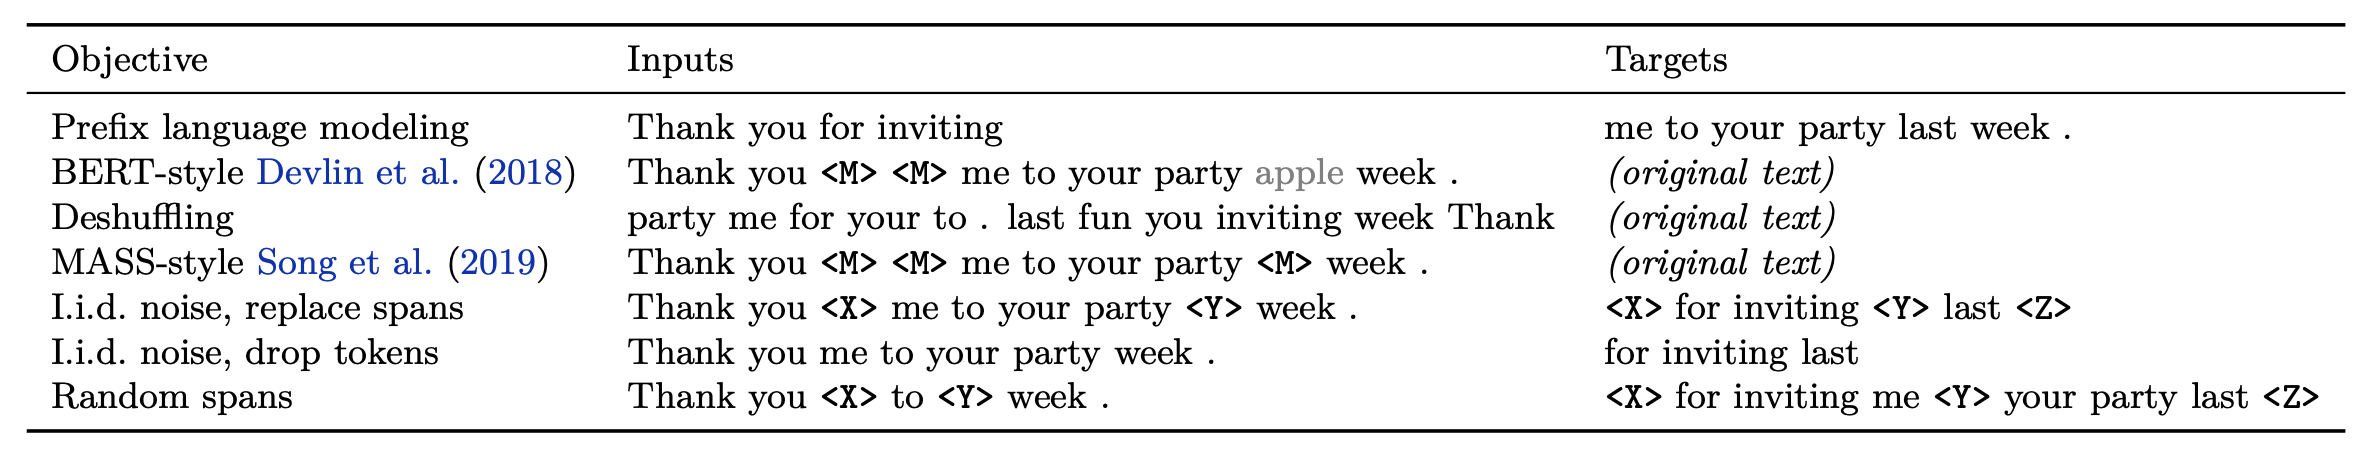
\includegraphics[width=1\textwidth]{images/imagen/t5_objectives.png}
    \caption{The unsupervised training objectives of T5 model. \textless M\textgreater\ denotes shared mask token (the same mask token is used to represent all masked positions in the input). \textless X\textgreater, \textless Y\textgreater, and \textless Z\textgreater\ denote sentinel tokens (with unique token IDs, they mark specific masked positions that the model should reconstruct).}
\end{figure}















\subsection{Pretrained text encoders}

In the paper, the researchers explored some of the biggest and most advanced text encoders: \textbf{T5-XXL} \cite{t5_model}, \textbf{GPT} \cite{gpt} \cite{mingpt} \cite{gpt_another}, and \textbf{BERT} \cite{bert}. These large language models (LLMs) are trained exclusively on text datasets, which are substantially larger compared to image-text pair datasets (as used in models like \textbf{CLIP}). Additionally, these models serve as significantly larger text encoders than those designed to handle image-text pairs alone.

Freezing these models \footnote{When we freeze models we generally mean that some (or all) of the parameters of the model are not changed during training. How? When a layer is frozen during training, no gradient updates will occur for this layer. Gradients will still flow from frozen layer to non-frozen layer, it doesn't skip the backpropogation. It just passes the gradients from the next layer to the previous layer.} (pre-training) provides significant advantage over training them: less memory and computation consumption during training (of the text-to-image model). They also found that scaling the text encoder size improves the quality of the generated images.














\subsection{Diffusion guidance weight}
\label{subsec:imagen_diffusion_guidance_weight}

As described before (section \ref{subsec:classifier_free_diffusion_guidance}), there are two methods to increase sample quality with the tradeoff of diversity:

\begin{itemize}
    \item \textbf{Classifier guidance} uses a separate, pre-trained classifier model to guide the image generation process in diffusion models by adjusting the noise based on how closely the generated image matches a desired condition.
    
    \item \textbf{Classifier-free guidance} (CFG) removes the need for a separate classifier by training the diffusion model itself to optionally condition on the label or text input, enabling the model to guide the generation internally, improving efficiency and reducing computational complexity.
\end{itemize}

More formally, in CFG, sampling is performed weighting the conditional and unconditional signals:

\begin{equation}
    \underbrace{\tilde{\epsilon}_\theta (z_t, c)}_{\text{adj noise prediction}} = \underbrace{w \epsilon_\theta (z_t, c)}_{\text{conditional score}} + \underbrace{(1 - w) \epsilon_\theta (z_t)}_{\text{unconditional score}}
    \label{eq:classifier_free_guidance}
\end{equation}

where $\epsilon_\theta$ is the noise prediction with the learned parameters $\theta$, $w$ is the \textbf{guidance weight} (conditional weight), $c$ is the condition, and $z_t$ is the latent variable at timestep $t$.

When $w=1$ the classifier-free guidance is disabled, and when $w>1$ it strengthens it. Imagen depends on this for effective text conditioning. The researchers conducted experiments and found that increasing the guidance weight improves image-text alignment but reduces image fidelity, producing unnatural images. Its caused by \textbf{train-test mismatch}: looking at equation \ref{eq:classifier_free_guidance} if we set $w$ to 1, then we disable classifier-free guidance, and then the model won't be trained on unconditional samples (only on conditional signals). This causes the model to generate outputs that exceed the noise prediction (in the paper they refer to this as "x-prediction") in the normalized range of [-1, 1]. And when iteratively applying the model to its own outputs at each step, errors caused by this mismatch accumulate, which causes unnatural artifacts in output images. When we set $w>1$ then it improves the model's image-text alignment, but damanges image fidelity by over-relying on conditional information.

For this reason they investigated static thresholding and dynamic thresholding.

\textbf{Static thresholding} is a method of applying the clipping operation to force the x-prediction output to fit to the normalized range of [-1, 1]. However, static thresholding still result in over-saturated and less detailed images as the guidance weight approaches 1.

\textbf{Dynamic thresholding} is a new sampling technique developed by the researchers. Instead of clipping the x-prediction to the normalized range, dynamic thresholding sets a threshold $s$ based on the distribution of absolute pixel values in the current x-prediction, allowing the threshold to adapt to the specific output of the model at that moment. In other words, if the pixel values are saturated (close to the [-1, 1] range), dynamic thresholding pushes them inwards by thresholding in the range [-$s$, $s$] and then dividing by $s$.

\begin{figure}
    \centering
    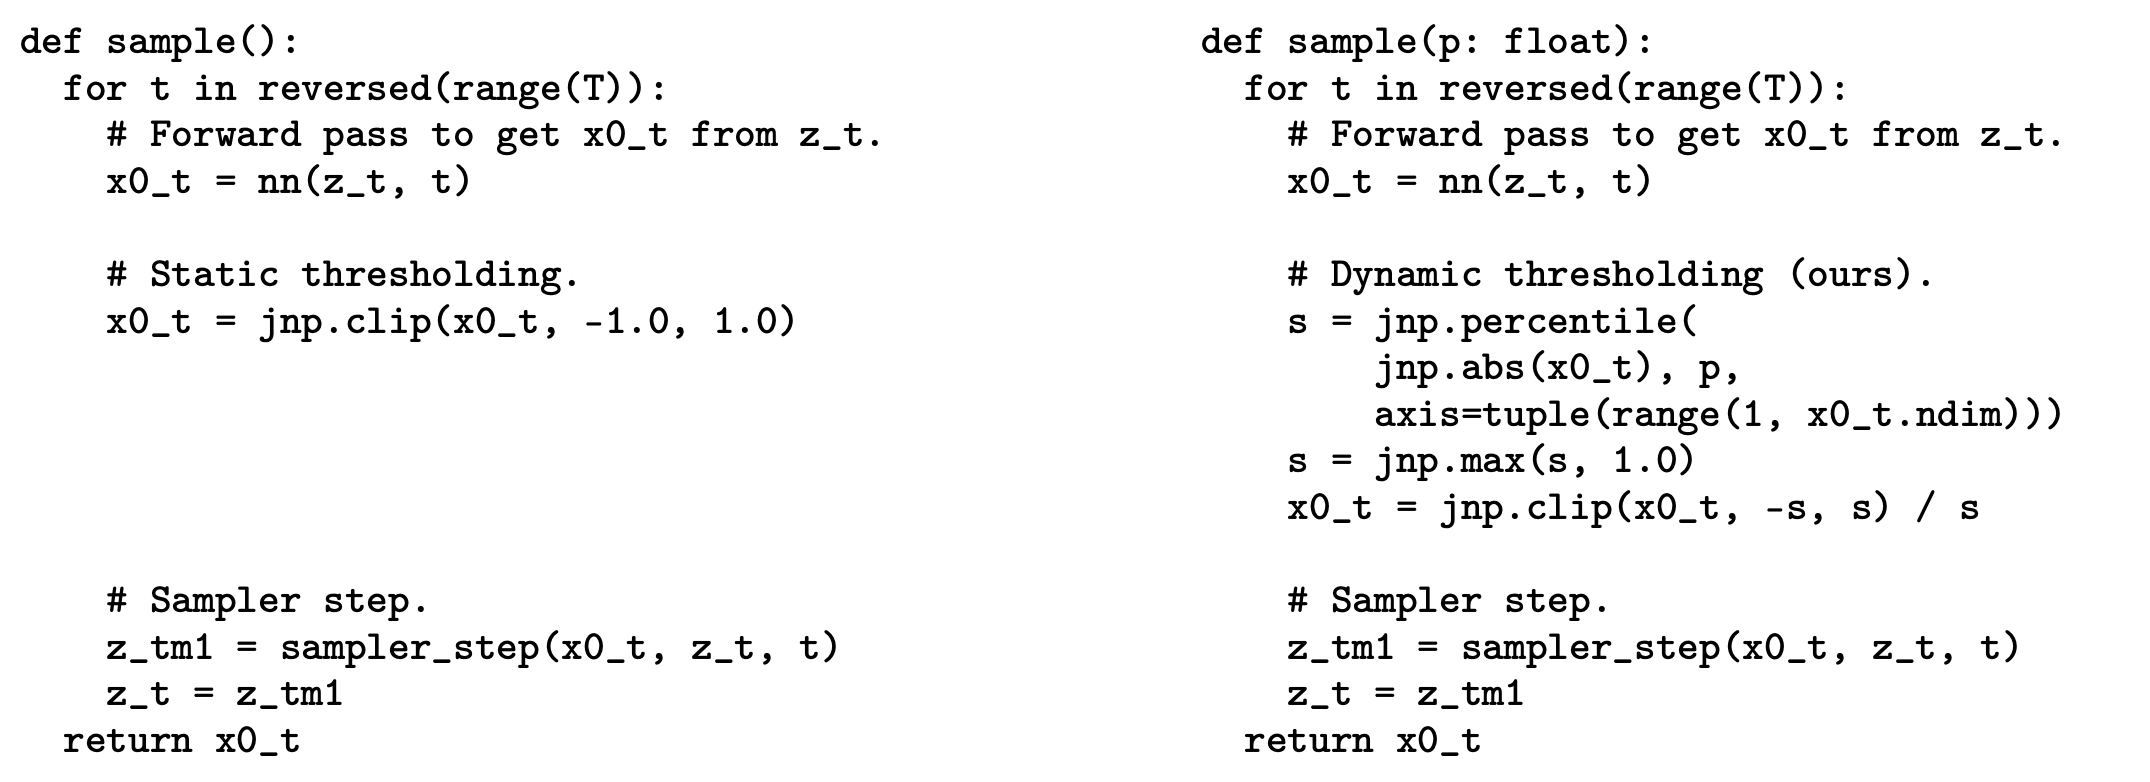
\includegraphics[width=0.75\textwidth]{images/imagen/static_dynamic_thresholding.png}
    \caption{Static (left) and dynamic (right) thresholding code implementation.}
    \label{fig:imagen_dynamic_thresholding}
\end{figure}

\begin{figure}
    \centering
    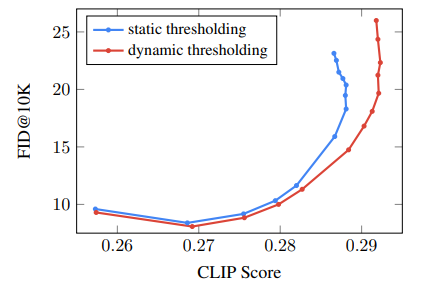
\includegraphics[width=0.4\textwidth]{images/imagen/static_vs_dynamic_thresholding.png}
    \caption{Static vs dynamic thresholding. Dynamic thresholding produces samples with more photorealism and image-text alignment over static thresholding.}
    \label{fig:imagen_static_vs_dynamic_thresholding}
\end{figure}

The implementation of static and dynamic thresholding is shown in figure \ref{fig:imagen_dynamic_thresholding}. The impact of dynamic thresholding is shown in figure \ref{fig:imagen_static_vs_dynamic_thresholding} where dynamic thresholding is shown to have more impact on FID as CLIP score increases.
















\subsection{Super-resolution via Repeated Refinment (SR3)}

\label{subsec:imagen_sr3}

In a 2021 paper \cite{sr3}, the Google Research team introduced a brand new concept: the use of diffusion models to upsample (super-resolution) images in iterative manner. Super-Resolution via Repeated Refinment (SR3) uses modified U-Net architecure in order to achieve the super-resolution task. Imagen builds upon this concept. The SR3 model upsamples 64x64 images to 256x256 and then to 1024x1024 via iterative refinement.

SR3 achieves close to a 50\% fool rate (47\%) \footnote{A 50\% fool rate means humans can't distinguish between a generated face image and an image of a real face.} on 16x16 $\rightarrow$ 128x128 faces, outperforming the previous state-of-the-art GAN models (FSRGAN and PULSE).

\textbf{Iterative refinment}: The input of the SR3 model is a low resolution image $x_{low}$, then the model applies \textbf{bicubic interpolation} \footnote{Bicubic interpolation is a method for resizing images that uses the closest 4x4 pixels grid to estimate new values, resulting in smoother transitions (compared to nearest-neighbor or bilinear interpolation) and fewer visual artifacts.} to upscale the image to the target resolution to get a higher-resolution image $x$ (however this creates artficats, large pixels), and then concatenates $x$ with a pure Gaussian noise $y_t \sim \mathcal{N} (0, I)$ channel-wise (see figure \ref{fig:sr3_architecture}). Then the U-Net iteratively refines the image $(x, y_t)$ by denoising. The output of a single refinement step is $y_{t-1}$. Then in the next refinement step, $x$ (which is unchanged) is concatenated with $y_{t-1}$ and the process is repeated until we reach $y_0$. The final output is a high-resolution image $y_0$. Note that both $x$ (after the upsampling), $y_t$ and the model's output are all the same resolution.

\textbf{The archirecture of SR3} is similar to the U-Net found in DDPM but with some modifications to the U-Net: they replaced the original DDPM residual blocks with residual blocks from BigGAN \cite{biggan_deep}, rescaled skip connections by $\frac{1}{\sqrt{2}}$, increased the number of residual blocks, and increased the number of the channel multipliers \footnote{Channel multipliers in a U-Net are the scaling factors used to adjust the number of feature channels at different U-Net layers. In other words, they increased the depth of the features at the cost of decreasing resolution at the convolution layers (down convolution, up convolution layers)} at different resolutions.

\begin{table}[h!]
    \centering
    \begin{tabular}{|l|m{8cm}|}
        \hline
        \textbf{Prior to Super Resolution} & \textbf{Limitations} \\ \hline
        Autoregressive Models           & Computationally expensive; Limited resolution \\ \hline
        Variational Autoencoder         & Sub-optimal sample quality \\ \hline
        Generative Adversarial Network  & Difficult to optimize; Requires additional functions to prevent instability \\ \hline
    \end{tabular}
    \caption{Related works to super-resolution to SR3 and their limitations compared to SR3.}
\end{table}


\begin{figure}
    \centering
    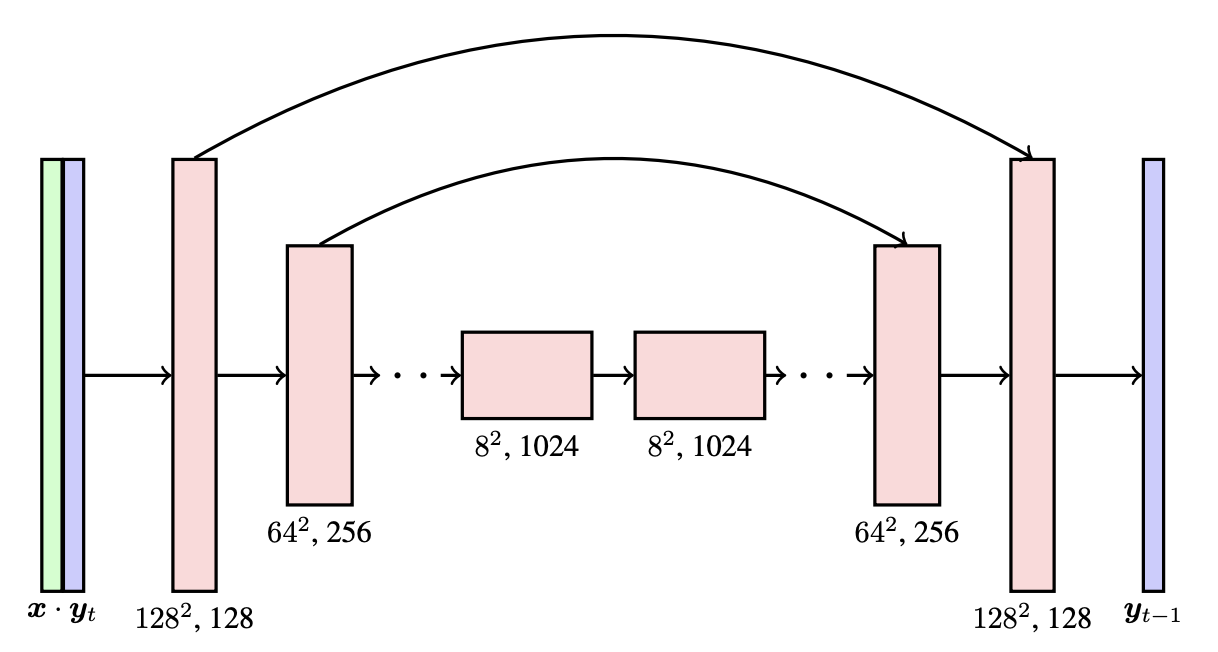
\includegraphics[width=0.75\textwidth]{images/imagen/sr3_architecture.png}
    \caption{A super-resolution model in SR3 for 16x16 $\rightarrow$ 128x128 image generation. Its a U-Net with skip connections, where $x$ is the input image (from previous model), which is upscaled to the target resolution using bicubic interpolation, and then its concatenated with the noise $y$.}
    \label{fig:sr3_architecture}
\end{figure}















\subsection{Cascaded diffusion models (CDMs)}

Cascaded diffusion models method was introduced in a 2022 paper \cite{cascaded_diffusion_models} also by Google Research. The Google Research team builds upon the SR3 paper \cite{sr3} and introduces a new method for super-resolution called Cascaded Diffusion Models (CDMs). The paper introduced class-conditioned ImageNet image generation with cascading models.

A cascaded diffusion model is compromised of a pipeline of multiple super-resolution diffusion models that generate images of increasing resolution, progressively upsample the image and add higher resolution details. The 2022 paper \cite{cascaded_diffusion_models} outperformed VQ-VAE 2 \cite{vqvae2} and BigGAN-deep \cite{biggan_deep} in FID metric on ImageNet dataset.

The 2022 paper \cite{cascaded_diffusion_models} uses the same architecture as SR3 paper \cite{sr3}. A base diffusion model generates data at a low resolution, followed by a sequence of SR3 super-resolution diffusion models that gradually increase the resolution of the generated images until we reach the target resolution.

A big strength of CDMs is the ability to train and fine tune each model individually, and then freezing their parameters.

\textbf{Conditioning augmentation} is the main and critical part of the paper \cite{cascaded_diffusion_models}. The researchers introduced this technique for super-resolution models, which allows to generate higher quality images with higher FID scores, compared to cascaded DDPMs without conditioning augmentation. The low-resolution base model may not be of sufficiently high quality in comparison to the original images in the training stage\footnote{While the super-resolution models in CDM are trained on original images from the dataset, during generation they need to perform super-resolution on the images generated by a low-resolution base model, which may not be of sufficiently high quality in comparison to the original images.}. This leads to \textbf{train-test mismatch} for the super-resolution models. Conditioning augmentation involves using data augmentation techniques on the low-resolution input image for each super-resolution model in a cascaded pipeline. In this process, augmentations such as Gaussian noise and Gaussian blur are applied to the input. This helps prevent each super-resolution model from overfitting to the low-resolution input, ultimately improving the quality of the higher-resolution outputs in the CDM.

\begin{figure}
    \centering
    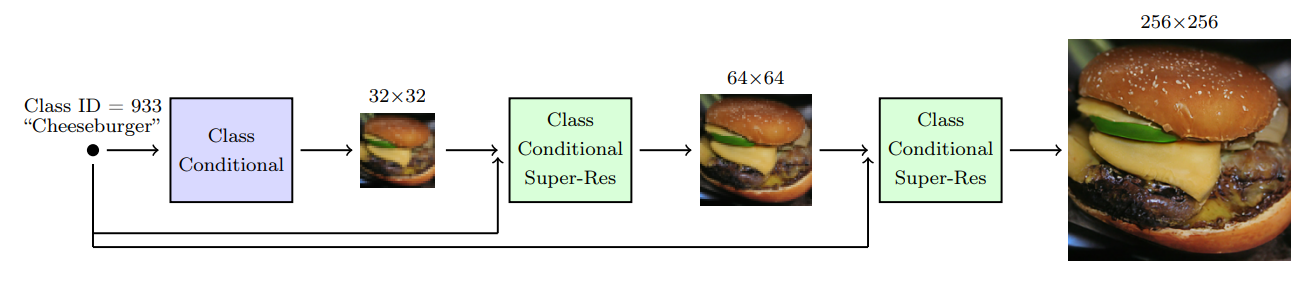
\includegraphics[width=0.75\textwidth]{images/imagen/cdm_architecture.png}
    \caption{Cascaded diffusion models (CDMs) architecture proposed in the 2022 paper \cite{cascaded_diffusion_models}. Notice the model is conditioned on class ID (label of cheeseburger).}
    \label{fig:imagen_cdm_architecture}
\end{figure}

Imagen, compared to SR3 \cite{sr3} and 2022 paper \cite{cascaded_diffusion_models} is a text-to-image diffusion model. SR3 wasn't designed for text conditioning and the 2022 paper \cite{cascaded_diffusion_models} was trained on class labels. See figure \ref{fig:imagen_cdm_architecture} for an overview of CDMs architecture proposed in the paper.

































\subsection{Architecture}

An overview of Imagen architecture is shown in figure \ref{fig:imagen_architecture}.

The researchers conducted experiments with frozen large language models such as BERT \cite{bert}, T5 \cite{t5_model}, and CLIP \cite{openai_clip} and found that humans prefer T5-XXL over CLIP.

The text encoder consists of a T5-XXL (T5-Extra Extra Large) text encoder, which maps text prompts (as conditioning signal) to embeddings. The T5-XXL model has 11 billion parameters, and its the largest version of the T5 model. All the diffusion models are conditioned on the same text embeddings.

\textbf{Base model}: the base model is 64x64 text-to-image diffusion model. The network is conditioned on text embeddings (via cross-attention and layer normalization layers), as well as with diffusion timestep embeddings, similar to the class embeddings in the 2022 paper \cite{cascaded_diffusion_models} and LDM (Stable Diffusion).

\textbf{Super-resolution models}: they used modified U-Net based on Improved DDPM paper \cite{openai_improved_ddpm} by OpenAI, specifically for the super-resolution models, since they deal with higher-dimensional data. By improving the U-Net they achieved 2-3x faster inference and convergence speed; they call this variant "Efficient U-Net". For the 256x256 $\rightarrow$ 1024x1024 super-resolution model, they removed self-attention layers but keep the cross-attention layers.

\textbf{Efficient U-Net}: is a new U-Net architectural variant for super-resolution models. Its more memory efficient and \textbf{2-3x faster in training and inference time}. There are several modifications to the U-Net architecture:

\begin{enumerate}
    \item \textbf{Residual blocks}: adding more residual blocks for lower resolutions, since lower-resolution images typically have more channels. They used 8 residual blocks at lower-resolution compared to typical 2-3 residual blocks used in standard U-Net.
    \item \textbf{Scaling the skip connections} by $\frac{1}{\sqrt{2}}$, similar to SR3 \cite{sr3}, significantly improves convergence speed.
    \item \textbf{Reversing order of downsampling and upsampling blocks}: In a standard U-Net, in in the downsampling block, downsampling occurs after the convolution layers, and in the upsampling block, upsampling is done before the convolutions. They reverse this order for both blocks which significantly improves the forward pass without performance degradation.
\end{enumerate}

The efficient U-Net architecture for 64x64 $\rightarrow$ 256x256 is shown in figure \ref{fig:imagen_efficient_unet}.

\begin{figure}
    \centering
    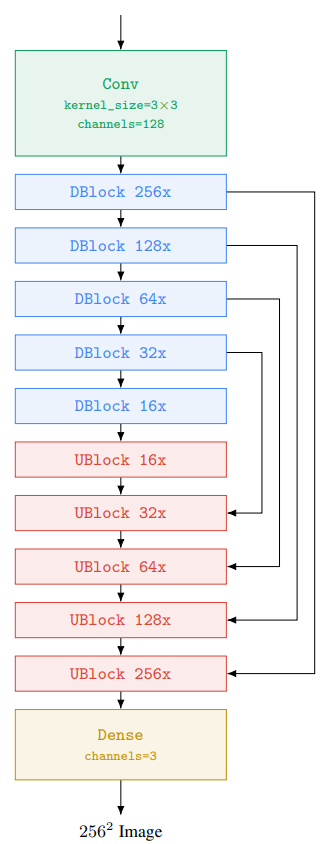
\includegraphics[width=0.25\textwidth]{images/imagen/efficient_unet.png}
    \caption{Efficient U-Net architecture for 64x64 $\rightarrow$ 256x256 super-resolution diffusion model, proposed in Imagen \cite{imagen}.}
    \label{fig:imagen_efficient_unet}
\end{figure}

Similar to Stable Diffusion / Latent Diffusion Models (LDMs), Imagen also uses classifier-free guidance \cite{classifier_free_guidance} (section \ref{subsec:classifier_free_diffusion_guidance}). Imagen depends critically on classifier-free guidance for effective text conditioning.

\begin{figure}
    \centering
    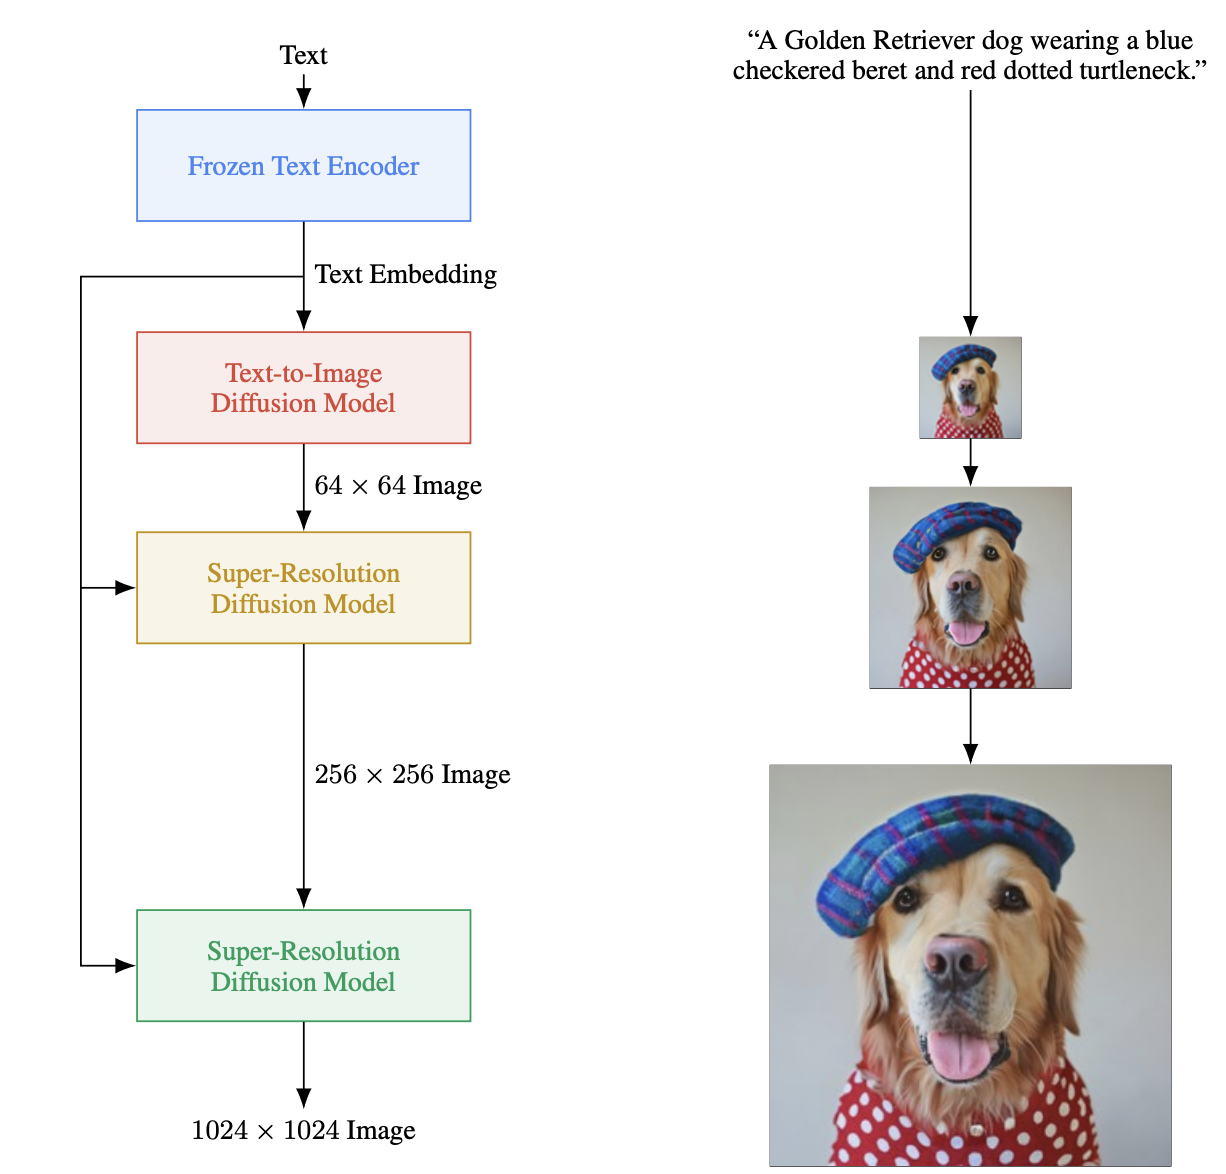
\includegraphics[width=0.5\textwidth]{images/imagen/architecture.png}
    \caption{Overview of Imagen architecture.}
    \label{fig:imagen_architecture}
\end{figure}

\textbf{Noise conditioning}: Imagen corrupts the 64x64 image with Gaussian noise. The amount of noise is random at training but arbitrary at inference time. They control the amount of corruption with \textit{aug\_level}, and the super-resolution model is conditioned on the augmentation level.

\textbf{Number of parameters}: the base model (64x64 text-to-image synthesis) has 2 billion parameters. The 64x64 $\rightarrow$ 256x256 super-resolution model has 600 million parameters, and the 256x256 $\rightarrow$ 1024x1024 super-resolution model has 400 million parameters. The size of the T5-XXL text encoder is 4.6 billion parameters.

\begin{figure}
    \centering
    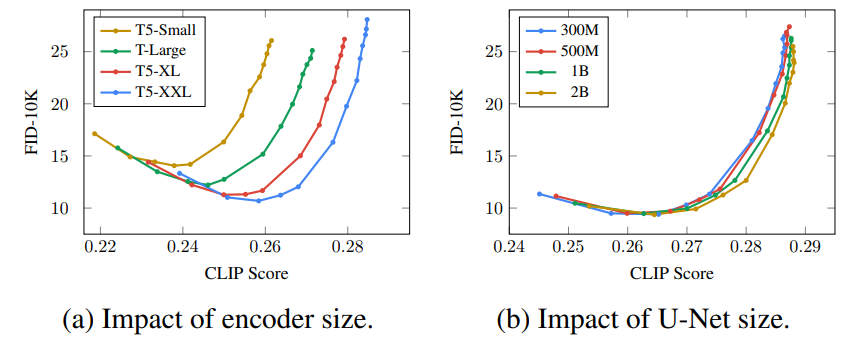
\includegraphics[width=0.75\textwidth]{images/imagen/encoder_vs_unet_size_impact.png}
    \caption{Scaling the encoder size is more impactful than scaling the U-Net size.}
    \label{fig:imagen_scaling_encoder_more_impactful_than_unet_scaling}
\end{figure}

\textbf{Scaling text encoder size is more important than U-Net size}: the researchers found that scaling text encoder (T5-XXL for example) is significantly more impactful than increasing U-Net size. See figure \ref{fig:imagen_scaling_encoder_more_impactful_than_unet_scaling} for reference.



% DBlock, UBlock

\begin{figure}
    \centering
    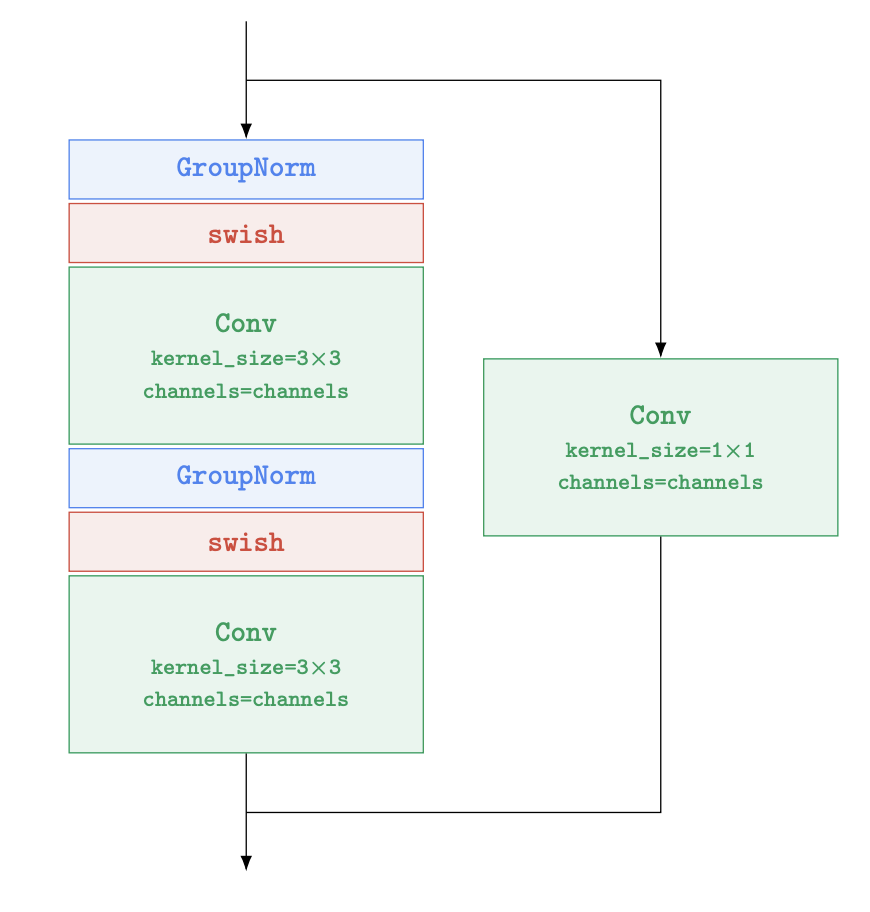
\includegraphics[width=0.4\textwidth]{images/appendix/imagen/unet_resnetblock.png}
    \caption{Imagen efficient U-Net \texttt{ResNetBlock} architecture.}
    \label{fig:imagen_resnetblock}
\end{figure}

In figure \ref{fig:imagen_resnetblock} we can see the \texttt{ResNetBlock} which is in use by both the \texttt{DBlock} (downsampler) and the \texttt{UBlock} (the upsampler). The only input of the \texttt{ResNetBlock} is the number of channels. The activation function is Swish (equation \ref{eq:appendix_activations_swish}). 

\begin{figure*}
    \centering
    \begin{subfigure}[b]{0.5\textwidth}   
        \centering 
        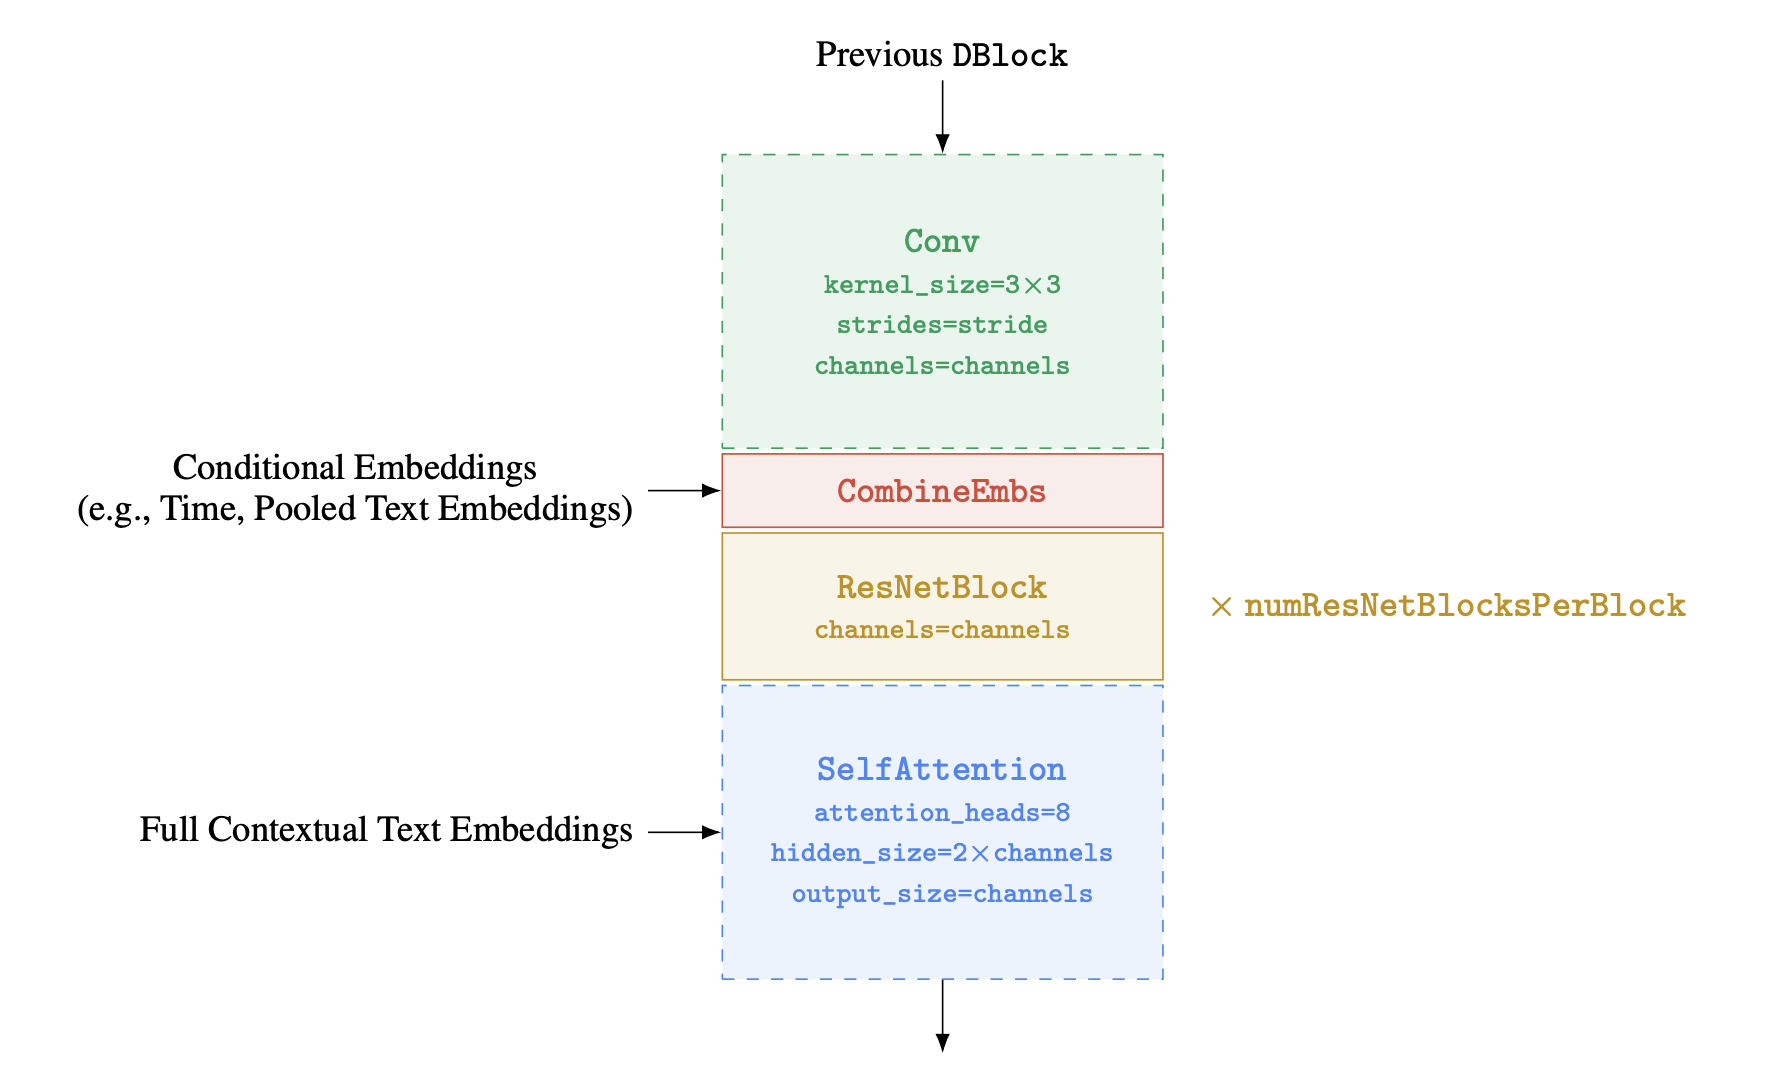
\includegraphics[width=\textwidth]{images/appendix/imagen/dblock.png}
        \caption[]%
        {{\small Imagen efficient U-Net \texttt{DBlock} architecture.}}
    \end{subfigure}
    \hfill
    \begin{subfigure}[b]{0.475\textwidth}
        \centering
        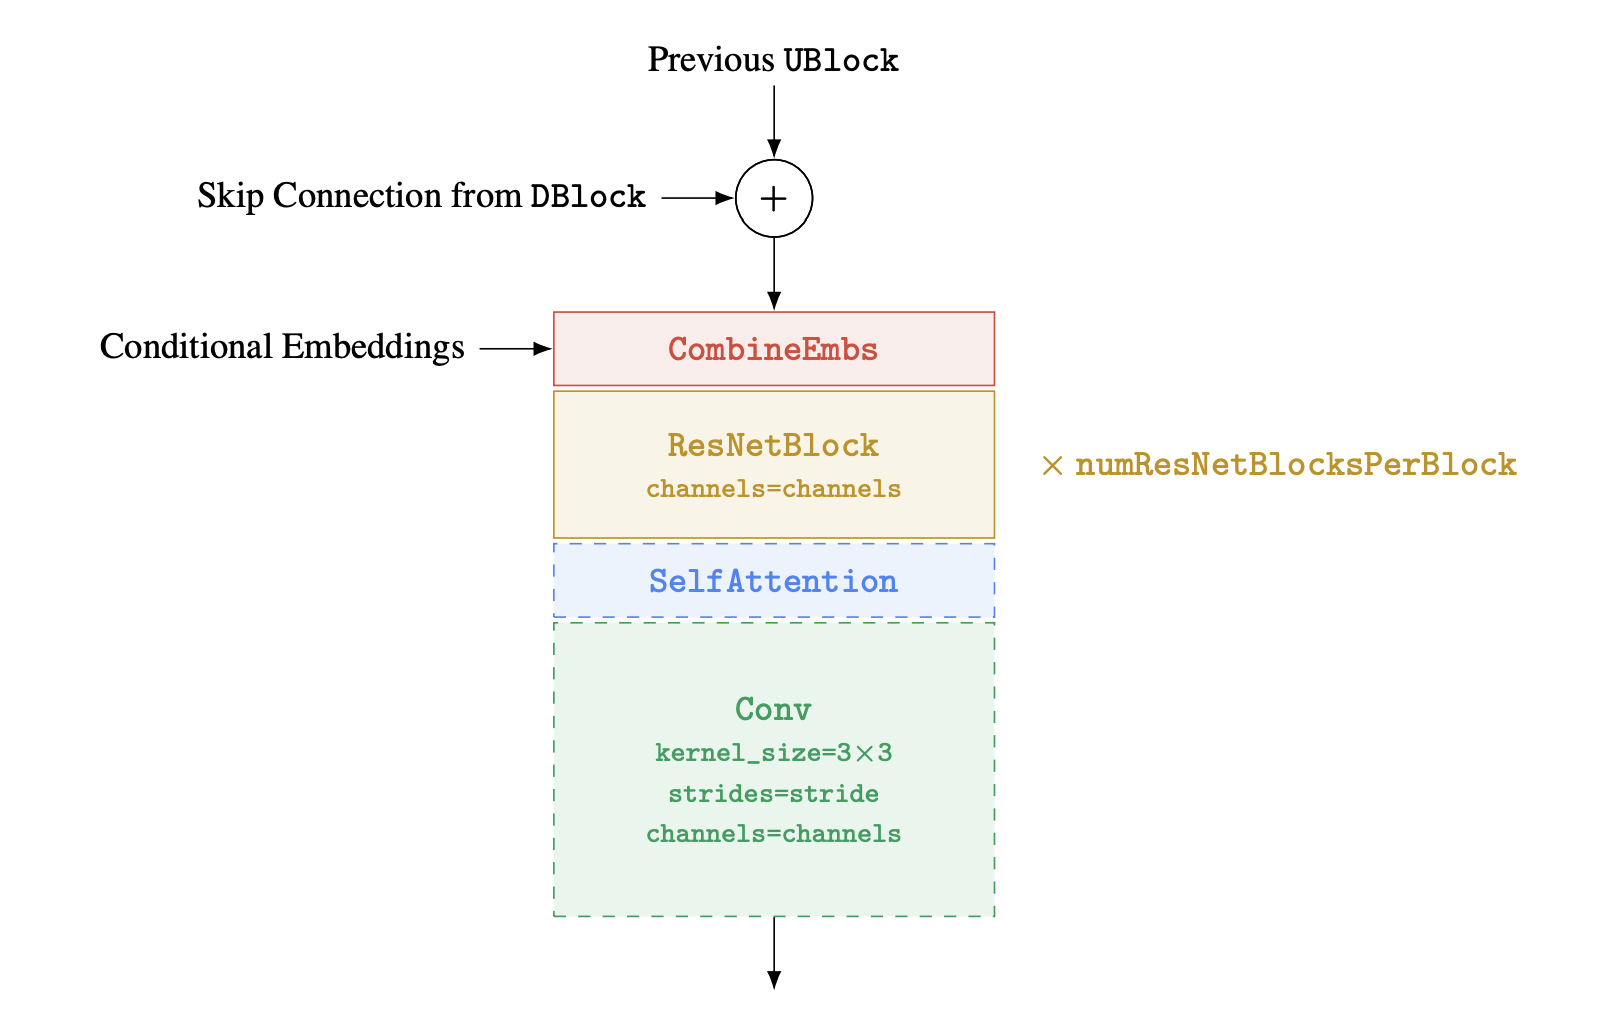
\includegraphics[width=\textwidth]{images/appendix/imagen/ublock.png}
        \caption[]%
        {{\small Imagen efficient U-Net \texttt{UBlock} architecture.}}
    \end{subfigure}
\end{figure*}















\subsection{DrawBench}

The COCO dataset \cite{coco_dataset} is a standard benchmark for evaluating text-to-image models. The standard performance metrics used are FID \cite{fid_score} which measure image fidelity (but is not fully aligned with perceptual quality \cite{perceptual_quality}), and CLIP score \cite{openai_clip} which measures image-text alignment (but is bad at counting objects in an image).

Due to these limitations, the researchers created new bnechmark called \textbf{DrawBench} that uses human evaluation to assess image quality by asking the question "Which image is more photorealistic (looks more real)?" and text-image alignment by asking the question "Does the caption accurately describe the above image?". For both cases they used 200 randomly chosen image-caption pairs from COCO dataset.

\begin{figure}
    \centering
    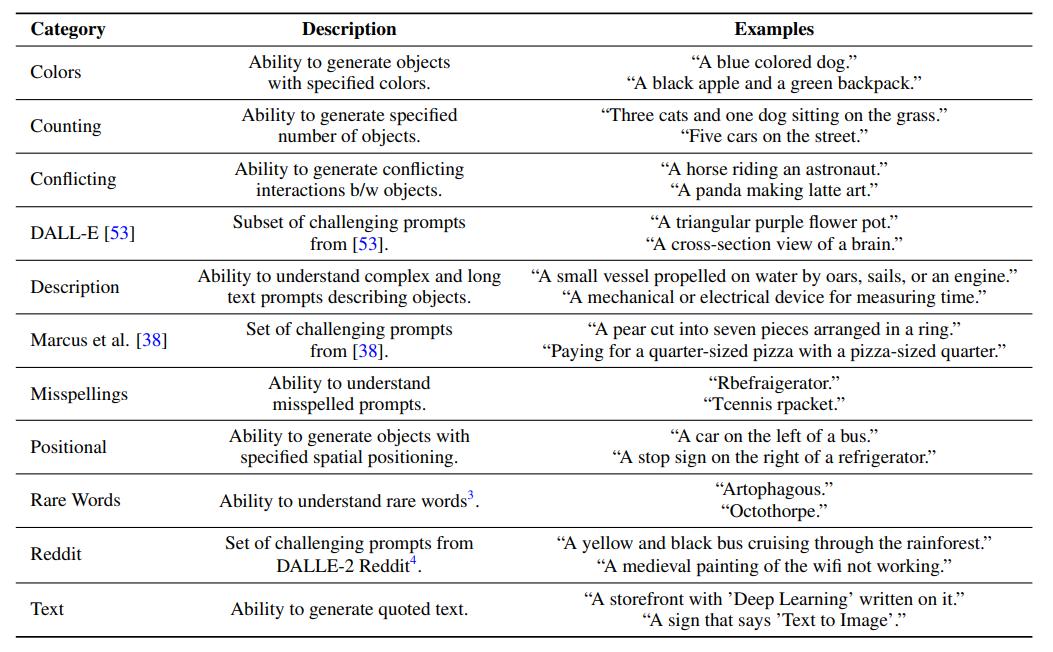
\includegraphics[width=0.75\textwidth]{images/imagen/drawbench_categories.png}
    \caption{Descriptions and examples of the 11 categories in DrawBench.}
    \label{fig:imagen_drawbench_categories}
\end{figure}

DrawBench has 11 categories of prompts which test different capabilities of models such as ability to render different colors, number of objects, spatial relations, text in the scene, and more. The prompts include long captions, rare words, and misspelled prompts. See figure \ref{fig:imagen_drawbench_categories} for examples of the categories and examples.














\subsection{Results}

\begin{figure}[t!]
    \centering
    \begin{subfigure}{0.4\textwidth}
        \centering
        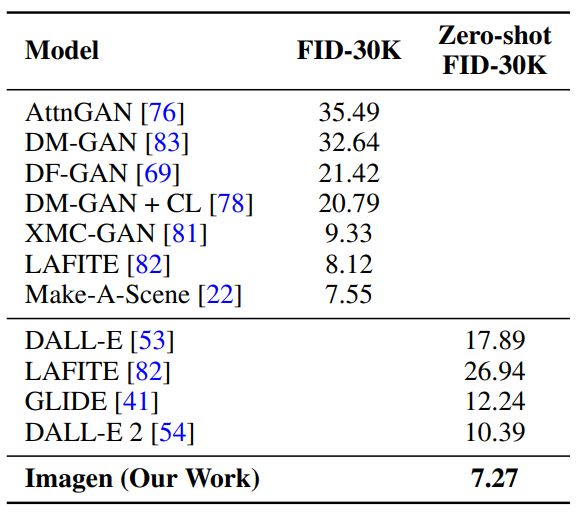
\includegraphics[width=0.6\linewidth]{images/imagen/imagen_coco_zeroshot.png}
        \caption{Although Imagen was not explicitly trained on MS-COCO dataset, it outperforms all other models on COCO FID score, achieving 7.27 FID.}
        \label{fig:imagen_coco_zeroshot}
    \end{subfigure}
    \begin{subfigure}{0.4\textwidth}
        \centering
        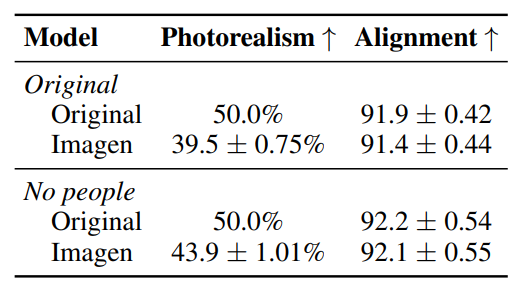
\includegraphics[width=0.6\linewidth]{images/imagen/imagen_coco_human_eval.png}
        \caption{Human evaluation on 256x256 COCO. Imagen splits to two categories: no filters, and human filters. Imagen struggles a little bit with photorealistic people.}
        \label{fig:imagen_coco_human_eval}
    \end{subfigure}
    \caption{Results of Imagen on COCO dataset.}
\end{figure}

\begin{figure}
    \centering
    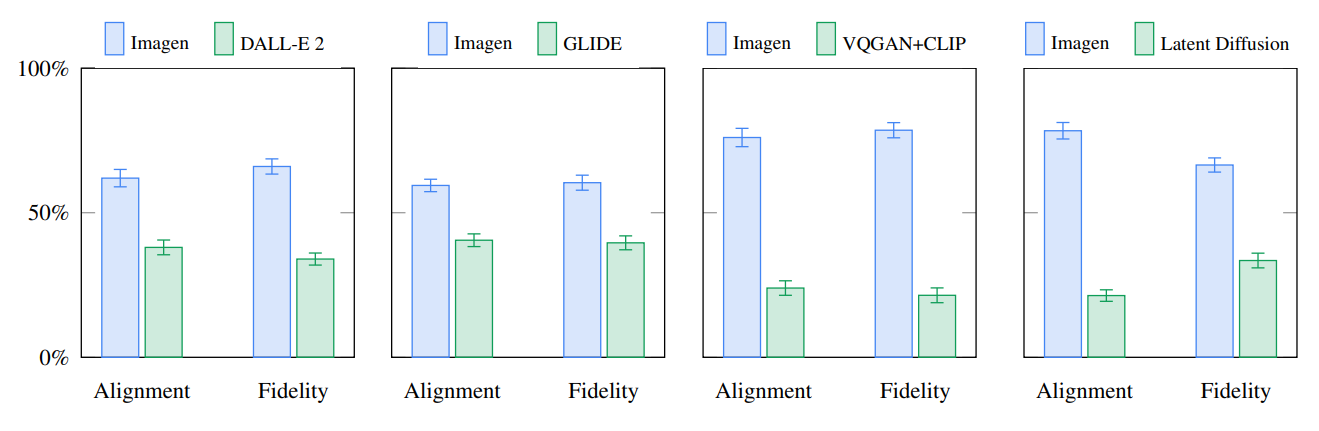
\includegraphics[width=0.75\textwidth]{images/imagen/alignment_fidelity_imagen_vs_models.png}
    \caption{Imagen beats all other models (DALL-E 2 \cite{dalle_2}, GLIDE \cite{glide}, VQGAN+CLIP \cite{vqgan_clip} and Latent Diffusion (Stable Diffusion) \cite{stable_diffusion} (section \ref{sec:stable_diffusion})) in terms of image-text alignment and image fidelity.}
    \label{fig:imagen_alignment_fidelity_vs_other_models}
\end{figure}

In figure \ref{fig:imagen_coco_zeroshot} we can see that although Imagen was not trained on the MS-COCO dataset, it still outperforms state-of-the-art models such as DALL-E 2 \cite{dalle_2} and achieves the best MS-COCO FID score of 7.27 in zero-shot setting.

In figure \ref{fig:imagen_coco_human_eval} we can see that Imagen achieves a respectable 43.9\% fool rate on 256x256 COCO human faces, indicating limited ability of Imagen to generate photorealistic people.

In figure \ref{fig:imagen_alignment_fidelity_vs_other_models} we can see that Imagen outperforms all other state-of-the-art models in terms of image fidelity and text-image alignment.
